\section{BẤT PHƯƠNG TRÌNH BẬC NHẤT HAI ẨN}
\subsection{LÝ THUYẾT CẦN NHỚ}
\subsubsection{Bất phương trình bậc nhất hai ẩn}
\indam{Bất phương trình bậc nhất hai ẩn:}
\begin{boxdn}
	Bất phương trình bậc nhất hai ẩn $x$, $y$ là bất phương trình có một trong các dạng sau
	\[ax + by < c,~ax + by > c,~ax + by \le c,~ax + by \ge c,\]
	trong đó $a$, $b$, $c$ là những số thực cho trước với $a$, $b$ không đồng thời bằng $0$; $x$, $y$ là các ẩn.
\end{boxdn}
\subsubsection{Miền nghiệm của bất phương trình bậc nhất hai ẩn}
\indam{Miền nghiệm:}
\begin{boxdn}
	Trong mặt phẳng  tọa độ $Oxy$, đường thẳng $d\colon ax+by=c$ chia mặt phẳng thành hai nửa mặt phẳng. Một trong hai nửa mặt phẳng (không kể $d$) là \textit{miền nghiệm} của bất phương trình $ax+by<c$, nửa mặt phẳng còn lại (không kể $d$) là \textit{miền nghiệm} của bất phương trình $ax+by>c$.
\end{boxdn}
\subsubsection{Biểu diễn miền nghiệm bất phương trình bậc nhất hai ẩn}
\indam{Phương pháp:}
\begin{boxdn}
	Các bước biểu diễn miền nghiệm của bất phương trình $ax+by<c$ trong mặt phẳng  tọa độ $Oxy$
	\begin{itemize}
		\item Bước 1. Vẽ đường thẳng $d\colon ax+by=c$. Đường thẳng $d$ chia mặt phẳng tọa độ thành hai nửa mặt phẳng.
		\item Bước 2. Lấy một điểm $M(x_0;y_0)$ không nằm trên $d$ (ta thường lấy gốc tọa độ $O$ nếu $c\ne0$). Tính $ax_0+by_0$ và so sánh với $c$.
		\item Bước 3. Kết luận
		\begin{itemize}
			\item Nếu $ax_0+by_0<c$ thì nửa mặt phẳng (không kể $d$) chứa điểm $M$ là miền nghiệm của bất phương trình $ax+by<c$.
			\item Nếu $ax_0+by_0>c$ thì nửa mặt phẳng (không kể $d$) không chứa điểm $M$ là miền nghiệm của bất phương trình $ax+by<c$.
		\end{itemize}
	\end{itemize}
\end{boxdn}
\subsection{PHÂN LOẠI VÀ PHƯƠNG PHÁP GIẢI TOÁN}
\begin{dang}{Biểu diễn miền nghiệm của một bất phương trình bậc nhất hai ẩn}
\begin{itemize}
	\item Bước 1. Vẽ đường thẳng $d\colon ax+by=c$. Đường thẳng $d$ chia mặt phẳng tọa độ thành hai nửa mặt phẳng.
	\item Bước 2. Lấy một điểm $M(x_0;y_0)$ không nằm trên $d$ (ta thường lấy gốc tọa độ $O$ nếu $c\ne0$). Tính $ax_0+by_0$ và so sánh với $c$.
	\item Bước 3. Kết luận
	\begin{itemize}
		\item Nếu $ax_0+by_0<c$ thì nửa mặt phẳng (không kể $d$) chứa điểm $M$ là miền nghiệm của bất phương trình $ax+by<c$.
		\item Nếu $ax_0+by_0>c$ thì nửa mặt phẳng (không kể $d$) không chứa điểm $M$ là miền nghiệm của bất phương trình $ax+by<c$.
	\end{itemize}
\end{itemize}
\end{dang}
\begin{vd}%[0D4B4-1]
	Biểu diễn miền nghiệm của bất phương trình $x+2y<3$.
	\loigiai{
		\immini
		{\begin{itemize}
				\item Vẽ đường thẳng $d\colon x+2y=3$.
				\item Lấy điểm $O(0;0)$. Ta có: $0+0=0<3$.
			\end{itemize}
			Vậy miền nghiệm của bất phương trình $x+2y<3$ là nửa mặt phẳng chứa điểm $O(0;0)$ không kể đường thẳng $d$ (nửa mặt phằng không bị gạch) (Hình bên).}
		{\begin{tikzpicture}[line cap=round,line join=round,font=\footnotesize,>=stealth,scale=1]
			\draw[->] (-1,0)--(4,0) node[above right] {$x$};
			\draw[->] (0,-1)--(0,3) node[left] {$y$};
			\fill (0,0) circle (1pt) node [below left] {$O$}; 
			\draw [samples=100, domain=-1:4] plot (\x, {(\x)/-2+3/2});
			\fill [pattern=north west lines] (-1,3)-- plot[domain=-1:4] (\x, {(\x)/-2+3/2})--(4,3)--(-1,3);
			\fill (3,0) node[shift={(-90:2ex)}]{$3$} circle(1pt)
			(0,1.5) node[shift={(-130:2ex)}]{$\dfrac{3}{2}$} circle(1pt)
			(-1,2) node[shift={(-80:2ex)}]{$d$} circle(0pt);
			\end{tikzpicture}}
	}
\end{vd}
\begin{vd}%[0D2H1-2]%
	[THPT Phan Ngọc Hiển- Cà Mau-GHKI NH23-24]
	Biểu diễn miền nghiệm của bất phương trình $x+y-2<0$ trong mặt phẳng tọa độ $Oxy$ và cho biết điểm $M(2023;2024)$ có thuộc miền nghiệm không?
	\loigiai{
		Vẽ đường thẳng $d\colon x+y-2=0$.\\
		Lấy điểm $O(0;0)\notin d$, ta có $0+0-2<0$ (đúng).\\
		Do đó miền nghiệm của bất phương trình đã cho là nửa mặt phẳng bờ $d$ chứa gốc tọa độ $O(0;0)$ (miền không bị gạch), không kể bờ $d$.
		\begin{center}
			\begin{tikzpicture}[line join=round, line cap=round,>=stealth,thick]
			\tikzset{every node/.style={scale=0.9}}
			\begin{scope}
			\clip (-2,-2) rectangle (3,4);
			\fill[pattern=north west lines] (-3,5)--(5,5)--(5,-3)--cycle;
			\draw (-2,4)--(4,-2) node [pos=0.45, above, sloped] {$x+y-2=0$};
			\end{scope}
			\draw[->] (-2,0)--(3,0) node[below]{$x$};
			\draw[->] (0,-2)--(0,4) node[left]{$y$};
			\draw (0,0) node[below left]{$O$};
			\end{tikzpicture}
		\end{center}
		Ta có $2023+2024-2=4045>0\Rightarrow$ Điểm $M(2023;2024)$ không thuộc miền nghiệm của bất phương trình.
	}
\end{vd}
\begin{dang}{Xác định bất phương trình bậc nhất hai ẩn tương ứng miền nghiệm cho trước}
	\begin{listEX}[1]
		\item [\ding{172}] Xác định phương trình đường thẳng chia mặt phẳng thành hai phần có dạng $ax+by=c$.
		\item [\ding{172}] Lấy một điểm $M(x_0;y_0)$ thuộc miền nghiệm của bất phương trình, thay tọa độ của điểm $M$ vào $ax+by$ rồi so sánh với $c$ để xác định bất phương trình cần tìm.
	\end{listEX}
\end{dang}

\begin{vd}%[0D4B4-1]
	\immini
	{Nửa mặt phẳng không bị gạch (không kể bờ $d$ ở hình bên) là miền nghiệm của bất phương trình nào?
	}
	{\begin{tikzpicture}[line cap=round,line join=round,font=\footnotesize,>=stealth,scale=1]
		\draw[->] (-1,0)--(4,0) node[above right] {$x$};
		\draw[->] (0,-2.5)--(0,2) node[left] {$y$};
		\fill (0,0) circle (1pt) node [below left] {$O$}; 
		\draw [samples=100, domain=-0.5:4] plot (\x, {(\x)-2});
		\fill [pattern=north west lines] (-1,-2.5)-- plot[domain=-0.5:4] (\x, {(\x)-2})--(4,2)--(-1,2);
		\fill (2,0) node[shift={(-90:2ex)}]{$2$} circle(1pt)
		(0,-2) node[shift={(-40:2ex)}]{$-2$} circle(1pt)
		(4,2) node[shift={(-80:2ex)}]{$d$} circle(0pt)
		(3,-1) node[shift={(-90:2ex)}]{$M$} circle(1pt)
		(3,0) node[shift={(90:2ex)}]{$3$} circle(1pt)
		(0,-1) node[shift={(180:2ex)}]{$-1$} circle(1pt);
		\draw[dashed](3,0)|-(0,-1);
		\end{tikzpicture}}
	\loigiai{
		Nhận thấy, đường thẳng đã cho có hệ số góc khác $0$.\\
		Gọi phương trình đường thẳng $d$ có dạng $y=ax+b$.\\
		Do đường thẳng $d$ đi qua điểm $(2;0)$ và $(0;-2)$ nên ta có
		$\heva{&2a+b=0\\&b=-2}\Leftrightarrow\heva{&a=1\\&b=-2.}$\\
		Vậy đường thẳng $d$ có phương trình $y=x-2$ hay $x-y=2$.\\
		Lấy điểm $M(3;-1)$ thuộc miền nghiệm của bất phương trình. Ta có: $3- (-1)=4>2$.\\
		Vậy nửa mặt phẳng không bị gạch (không kể $d$) ở hình bên là miền nghiệm của bất phương trình $x-y>2$.
	}
\end{vd}
\begin{vd}%[0D2N1-2]%
	[THPT Hai Bà Trung - TP. Huế-GHKI-NH23-24]
	Nửa mặt phẳng \textbf{không} bị gạch (kể cả $d$) là miền nghiệm của bất phương trình nào?
	\begin{center}
		\begin{tikzpicture}[scale=1.5, font=\footnotesize, line join=round, line cap=round, >=stealth]
		\draw[->]({-1},0)--({3},0)node[right]{$x$};
		\draw[->](0,{-1})--(0,{2})node[above]{$y$};
		\draw(0,0) node[below left]{$0$};
		\clip ({-1+0.1},{-1+0.1}) rectangle ({3-0.1},{2-0.1});
		\path [pattern=north east lines,pattern color = black,opacity=0.8] ({-1},{2})--plot[domain={-1}:{3}] (\x,{-1/2*\x+1})--({3},{2})--cycle;
		\draw plot[domain={-1}:{3}] (\x,{-1/2*\x+1});
		\draw[fill=black]
		(2,0) circle (0.04) node[below]{$2$}
		(0,1) circle (0.04) node[left]{$1$}
		;
		\end{tikzpicture}
	\end{center}
	\loigiai
	{
		Đường thẳng đi qua điểm $(2;0)$ và $(0;1)$ có phương trình $x+2y=2$.\\
		Điểm $(0;0)$ thuộc miền nghiệm của bất phương trình nên bất phương trình có dạng $x+2y\le0$.
	}
\end{vd}
\begin{dang}{Ứng dụng}
\end{dang}
\begin{vd}%[0D2H1-3]%
	[THPT Chuyên Lê Quý Đôn - Ninh Thuận - GHKI NH23-24]
	Một công ty dự định không chi quá $900$ triệu đồng để quảng cáo trên VTV. Biết rằng giá quảng cáo trên VTV là $30$ triệu đồng cho $1$ lần phát vào khung giờ $I$, và $6$ triệu đồng cho $1$ lần phát phát vào khung giờ $II$. Gọi $x$ và $y$ lần lượt là số lần phát quảng cáo vào khung giờ $I$ và $II$. Hãy thiết lập bất phương trình số tiền mà công ty này phải trả theo $x$ và $y$.
	\loigiai{
		Số tiền mà công ty phải trả trong khung giờ $I$ là $30x$ triệu đồng.\\
		Số tiền mà công ty phải trả trong khung giờ $II$ là $6y$ triệu đồng.\\
		Vì số tiền phải chi không vượt quá $900$ triệu nên ta có bất phương trình $30x+6y\leq 900$ triệu đồng.\\
		Hay $10x+2y\leq 300$.
	}
\end{vd}
\begin{vd}%[0D4B4-3]
	Một gian hàng trưng bày bàn và ghế rộng $60$ m$^2$. Diện tích để kê một chiếc ghế là $0{,}5$ m$^2$, một chiếc bàn là $1{,}2$ m$^2$. Gọi $x$ là số chiếc ghế, $y$ là số chiếc bàn được kê.
	\begin{enumerate}
		\item Viết bất phương trình bậc nhất hai ẩn $x$, $y$ cho phần mặt sàn để kê bàn và ghế, biết diện tích mặt sàn dành cho lưu thông tối thiểu là $12$ m$^2$.
		\item Chỉ ra ba nghiệm của bất phương trình trên.
	\end{enumerate}
	\loigiai{
		\begin{enumerate}
			\item Diện tích để kê $x$ chiếc ghế, $y$ chiếc bàn là $0{,}5x+1{,}2y$ (m$^2$).\\
			Diện tích tối đa để kê bàn và ghế là $60-12=48$ (m$^2$).\\
			Ta có bất phương trình: $0{,}5x+1{,}2y\le 48$ (m$^2$).
			\item Ba nghiệm có thể chỉ ra được của bất phương trình trên là $(20;30),~(30;20),~(50;15)$.
		\end{enumerate}
	}
\end{vd}
\subsection{BÀI TẬP RÈN LUYỆN}
\ind{PHẦN I.} \inden{Câu trắc nghiệm nhiều phương án lựa chọn. Mỗi câu hỏi học sinh chỉ chọn một phương án.}\\
\setcounter{ex}{0}
\Opensolutionfile{ans}[ans/2D1-Bai1-TN]%--Đặt tên 2D1-Bai1-Dang1-TN
%E:\Latex-Phong\Thu-ID6\AHV-2024-2025\SpDuAn-A-Dot4\SpDuAn-A-Dot4\data\GHKI\0-TL-TN-DS-THPT-NguyenThiMinhKhai-TpHCM-GHKI-NH24-25.tex
\begin{ex}%[0D2N1-1]%
	[THPT Nguyễn Thị Minh Khai  - Tp.HCM - GHKI-NH24-25]
	Trong các bất phương trình sau, bất phương trình nào là bất phương trình bậc nhất hai ẩn?
	\choice
	{$2x-5y+3z \leq 0$}
	{$3x^2+2x-4> 0$}
	{$2x^2+5y > 3$}
	{\True $2x+3y < 5$}
	\loigiai{
		Bất phương trình $2x+3y < 5$ là bất phương trình bậc nhất hai ẩn.
	}
\end{ex}
\begin{ex}%[0D2N1-1]%
	[Ôn tập giữa học kì 1 - Chuyên Lê Quý Đôn - Ninh Thuận - 24-25]
	Bất phương trình nào dưới đây \textbf{không} phải là bất phương trình bậc nhất $2$ ẩn?
	\choice
	{ $x+y-2 \geq 0$}
	{\True $2x+y-xy+2 \leq 0$}
	{$x+0y \leq 0$}
	{ $x-y-2 \geq 0$}
	\loigiai{
		Bất phương trình $2x+y-xy+2 \leq 0$ không phải là bất phương trình bậc nhất $2$ ẩn.
	}
\end{ex}
\begin{ex}%[0D2N1-1]%
	[Chuyên Lê Quý Đôn - Ninh Thuận - GHKII-NH24-25]
	Cặp số nào sau đây là nghiệm của bất phương trình $-2(x-y)+y>3$?
	\choice
	{\True $(-4 ; 4)$}
	{$(4 ;-4)$}
	{$(-1 ;-2)$}
	{$(2 ; 1)$}
	\loigiai{
		Thay $x=-4$; $y=4$ và  $-2(x-y)+y>3$ ta được $20>3$ (đúng) nên $(-4 ; 4)$ là nghiệm.
	}
\end{ex}
\begin{ex}%[0D2N1-1]%
	[THPT Trần Văn Giàu - GHKI-NH23-24]
	Trong các cặp số $(x; y)$ sau đây, cặp nào là nghiệm của bất phương trình $2 x+y<1$?
	\choice
	{$(3;7)$}
	{$(2;-1)$}
	{\True $(-2;1)$}
	{$(0;1)$}
	\loigiai{
		Với $(x;y)=(-2;1)$, ta có: $2x+y=2\cdot (-2)+1=-3<0$ (thỏa mãn) nên $(-2;1)$ là nghiệm của bất phương trình.
	}	
\end{ex}
%E:\Latex-Phong\Thu-ID6\SACH-CTST-K11-GOC\Sp dot 1,2,3\Tong hop\data\Dot1\0-TL-TN-THPT-Nguyen-Du-GHKI-NH23-24.tex
\begin{ex}%[0D2N1-2]%
	[THPT Nguyễn Du- Tp HCM - GHKI NH23-24]
	Điểm $A(5 ;-3)$ là điểm thuộc miền nghiệm của bất phương trình nào sau đây?
	\choice
	{\True $5x-2y+1 \geq 0$}
	{$x-2y<0$}
	{$-3x+y+2>0$}
	{$2x-3y \leq 0$}
	\loigiai{
		Thay $x=5$ và $y=-3$ vào từng bất phương trình:
		\begin{itemize}
			\item $5 \cdot 5 - 2 \cdot (-3) + 1 = 25 + 6 + 1 = 32 \geq 0$ (thỏa mãn)
			\item $5 - 2 \cdot (-3) = 5 + 6 = 11 > 0$ (không thỏa mãn)
			\item $-3 \cdot 5 + (-3) + 2 = -15 - 3 + 2 = -16 < 0$ (không thỏa mãn)
			\item $2 \cdot 5 - 3 \cdot (-3) = 10 + 9 = 19 \leq 0$ (không thỏa mãn)
		\end{itemize}
		Kết quả là $5x-2y+1 \geq 0$.
	}
\end{ex}

\begin{ex}%[0D2N1-2]%
	[THPT Hai Bà Trưng - TP. Huế - GHKI NH23-24]
	Miền nghiệm của bất phương trình $3 x-y>3$ được xác định bởi nửa mặt phẳng (phần \textbf{không} bị gạch, không kể $d$ ) nào sau đây?
	\choice
	{\begin{tikzpicture}[scale=1, font=\footnotesize, line join=round, line cap=round, >=stealth]
		\draw[->]({-1},0)--({4},0)node[right]{$x$};
		\draw[->](0,{-2})--(0,{2})node[above]{$y$};
		\draw(0,0) node[below left]{$O$};
		\clip ({-1+0.1},{-2+0.1}) rectangle ({4-0.1},{2-0.1});
		\path [pattern=north east lines,pattern color = black,opacity=0.8] ({-1},{2})--plot[domain={-1}:{4}] (\x,{1/3*\x+-1})--({4},{2})--cycle;
		\draw plot[domain={-1}:{4}] (\x,{1/3*\x+-1});
		\draw[fill=black]
		(3,0) circle (0.04) node[below]{$3$}
		(0,-1) circle (0.04) node[below right]{$-1$}
		;
		\end{tikzpicture}}
	{\True \begin{tikzpicture}[scale=1, font=\footnotesize, line join=round, line cap=round, >=stealth]
		\draw[->]({-1},0)--({3},0)node[right]{$x$};
		\draw[->](0,{-4})--(0,{1})node[above]{$y$};
		\draw(0,0) node[below left]{$0$};
		\clip ({-1+0.1},{-4+0.1}) rectangle ({3-0.1},{1-0.1});
		\path [pattern=north east lines,pattern color = black,opacity=0.8] ({-1},{1})--plot[domain={-1}:{3}] (\x,{3*\x+-3})--({3},{1})--cycle;
		\draw plot[domain={-1}:{3}] (\x,{3*\x+-3});
		\draw[fill=black]
		(1,0) circle (0.04) node[below right]{$1$}
		(0,-3) circle (0.04) node[right]{$-3$}
		;
		\end{tikzpicture}}
	{\begin{tikzpicture}[scale=1, font=\footnotesize, line join=round, line cap=round, >=stealth]
		\draw[->]({-1},0)--({3},0)node[right]{$x$};
		\draw[->](0,{-4})--(0,{1})node[above]{$y$};
		\draw(0,0) node[below left]{$0$};
		\clip ({-1+0.1},{-4+0.1}) rectangle ({3-0.1},{1-0.1});
		\path [pattern=north east lines,pattern color = black,opacity=0.8] ({-1},{-4})--plot[domain={-1}:{3}] (\x,{3*\x+-3})--({3},{-4})--cycle;
		\draw plot[domain={-1}:{3}] (\x,{3*\x+-3});
		\draw[fill=black]
		(1,0) circle (0.04) node[above left]{$1$}
		(0,-3) circle (0.04) node[left]{$-3$}
		;
		\end{tikzpicture}}
	{\begin{tikzpicture}[scale=1, font=\footnotesize, line join=round, line cap=round, >=stealth]
		\draw[->]({-1},0)--({4},0)node[right]{$x$};
		\draw[->](0,{-2})--(0,{2})node[above]{$y$};
		\draw(0,0) node[below left]{$0$};
		\clip ({-1+0.1},{-2+0.1}) rectangle ({4-0.1},{1-0.1});
		\path [pattern=north east lines,pattern color = black,opacity=0.8] ({-1},{-2})--plot[domain={-1}:{4}] (\x,{1/3*\x+-1})--({4},{-2})--cycle;
		\draw plot[domain={-1}:{4}] (\x,{1/3*\x+-1});
		\draw[fill=black]
		(3,0) circle (0.04) node[above]{$3$}
		(0,-1) circle (0.04) node[above left]{$-1$}
		;
		\end{tikzpicture}}
	\loigiai
	{
		Miền nghiệm của $3x-y>3$ là nửa mặt phẳng bờ là đường thẳng $3x-y=3$ đi qua hai điểm $(1;0)$ và $(0;-3)$ và không chứa điểm $(0;0)$ không kể cả bờ.
	}
\end{ex}

\begin{ex}%[0D2N1-2]%
	[THPT Chuyên Hùng Vương - Phú Thọ - GHKI-NH23-24]
	Bất phương trình bậc nhất hai ẩn nào có miền nghiệm như hình vẽ dưới đây (phần không tô đậm, kể cả đường thẳng)?
	\begin{center}
		\begin{tikzpicture}[>=stealth,line join=round,line cap=round,font=\footnotesize,scale=0.8]
		\draw[->,line width = 1pt] (-1.5,0)--(0,0) node[below left]{$O$}--(4.5,0) node[below]{$x$};
		\draw[->,line width = 1pt] (0,-1.8) --(0,5.4) node[right]{$y$};
		\fill (-1.2,0) node[below]{$-50$};
		\fill (-1,0) circle (1pt);
		\fill (1,0) node[below]{$50$} circle (1pt);
		\fill (2,0) node[above right]{$100$} circle (1pt);
		\fill (0,-1) node[left]{$-50$} circle (1pt);
		\fill (0,1) node[left]{$50$} circle (1pt);
		\fill (0,3) node[left]{$150$} circle (1pt);
		\draw [thick, domain=-1.5:3.2, samples=100] %d1
		plot (\x, {-1.5*(\x) + 3});
		\fill[opacity=.2,pattern= north east lines] (-1.5,5.25)--(4.5,5.25)--(4.5,-1.8)--(3.2,-1.8)--cycle;
		\end{tikzpicture}
	\end{center}
	\choice
	{$3x + 2y < 300$}
	{\True $3x + 2y \geq 300$}
	{$3x + 2y > 300$}
	{$3x + 2y \leq 300$}
	\loigiai{
		Xét $O(0;0) \notin (d)\colon 3x + 2y = 300$.\\
		Ta có $3\cdot 0 + 2\cdot 0 = 0 < 300$ nên bất phương trình bậc nhất hai ẩn $3x + 2y \geq 300$ có miền nghiệm như hình vẽ trên.
	}
\end{ex}
\begin{ex}%[0D2N1-2]%
	[THPT Quang Trung - Hải Dương - GHKI-NH22-23]
	Điểm nào sau đây thuộc miền nghiệm của bất phương trình $2x+y-3>0$?
	\choice
	{$Q\left (-1;-3 \right )$}
	{\True $M\left (1; \dfrac{3}{2} \right )$}
	{$N\left (1;1 \right )$}
	{$P\left (-1; \dfrac{3}{2} \right )$}
	\loigiai{
		Ta thấy $2\cdot1+\dfrac{3}{2}-2=\dfrac{1}{2}>0$. Do đó điểm $M$ thuộc miền nghiệm của bất phương trình $2x+y-3>0$.}
\end{ex}
\begin{ex}%[0D2H1-2]%
	[THPT Nguyễn Du - Tp.HCM -GHKI-NH23-24]
	Miền nghiệm của bất phương trình $3x + 2(y+3) \ge 4(x+1)-y+3$ chứa điểm nào trong các điểm sau?
	\choice
	{$A(3;1)$}
	{\True $B(2;1)$}
	{$C(3;0)$}
	{$O(3;0)$}
	\loigiai{
		Thay tọa độ các điểm vào bất phương trình đã cho ta thấy điểm $B(2;1)$ thỏa mãn.
	}
\end{ex}
\begin{ex}%%[0D2H1-3]%
	[THPT  Nguyễn Thượng Hiền - Tp. HCM - GHKI-NH23-24]
	Một hãng taxi có bảng giá cho xe 4 chỗ như sau$\colon$
	
	\vspace{5pt}
	\begin{tabular}{|c|c|c|}
		\hline \begin{tabular}{c} 
			Giá mở cửa \\
			(Từ 1 kilômét trở xuống)
		\end{tabular} & \begin{tabular}{c} 
			Giá cước\\
			các kilômét tiếp theo
		\end{tabular} & Giá cước từ kilômét thứ 31 \\
		\hline 11000 đồng & 15000 đồng & 12000 đồng \\
		\hline
	\end{tabular}
	\vspace{5pt}
	
	Một hành khách thuê xe taxi đi quãng đường $x$ kilômét phải trả số tiền là $y$ nghìn đồng. Hãy biểu diễn $y$ theo $x$ biết người này đi từ thành phố Hồ Chí Minh đến tỉnh Bình Dương có khoảng cách trên 30 kilômét.
	\choice
	{$y=12000 x+86000$}
	{$y=12000 x+90000$}
	{$y=12 x+90$}
	{\True $y=12 x+86$}
	\loigiai{Số tiền phải trả trong $1$ km đầu tiên là$\colon$ $11$ (nghìn đồng).\\
		Số tiền phải trả từ 1 - 30 km tiếp theo là$\colon$ $29 \cdot 15 = 435$ (nghìn đồng).\\
		Số tiền phải trả những km tiếp theo là$\colon$ $(x-30) \cdot 12 =12x-360$ (nghìn đồng).\\
		Vậy tổng số tiền phải trả là$\colon$ $11 + 435 + 12x-360 = 12x +86$ (nghìn đồng).}
\end{ex}
\begin{ex}%%[0D2N1-2]
	Miền nghiệm của bất phương trình $2x-3y>5$ là nửa mặt phẳng (không kể đường thẳng $d\colon 2x-3y=5$) không chứa điểm có toạ độ nào sau đây?
	\choice
	{\True $(0;0)$}
	{$(3;0)$}
	{$(1;-2)$}
	{$(-3;-4)$}
	\loigiai{
		Ta có $2\cdot0-3\cdot0=0<5$ nên miền nghiệm không chứa điểm $(0;0)$.
	}
\end{ex}
\begin{ex}%%[0D2H1-2]
	Miền nghiệm của bất phương trình $x-2y<4$ được xác định bởi miền nào (nửa mặt phẳng không bị gạch và không kể $d$) sau đây?
	\choice
	{\begin{tikzpicture}[line cap=round,line join=round,font=\footnotesize,>=stealth,scale=0.75]
		\draw[->] (-1,0)--(5,0) node[below] {$x$};
		\draw[->] (0,-2.5)--(0,1) node[left] {$y$};
		\fill (0,0) circle (1pt) node [below left] {$O$}; 
		\draw [samples=100, domain=-1:5] plot (\x, {(\x)/2-2});
		\fill [pattern=north west lines] (-1,1)-- plot[domain=-1:5] (\x, {(\x)/2-2})--(5,1)--(-1,1);
		\fill (4,0) node[shift={(-90:2ex)}]{$4$} circle(1pt)
		(0,-2) node[shift={(-40:2ex)}]{$-2$} circle(1pt)
		(5,0.5) node[shift={(0:1ex)}]{$d$} circle(0pt)
		;
		\end{tikzpicture}}
	{\True \begin{tikzpicture}[line cap=round,line join=round,font=\footnotesize,>=stealth,scale=0.75]
		\draw[->] (-1,0)--(5,0) node[below] {$x$};
		\draw[->] (0,-2.5)--(0,1) node[left] {$y$};
		\fill (0,0) circle (1pt) node [below left] {$O$}; 
		\draw [samples=100, domain=-1:5] plot (\x, {(\x)/2-2});
		\fill [pattern=north west lines] (5,-2.5)-- plot[domain=-1:5] (\x, {(\x)/2-2})--(5,-2.5);
		\fill (4,0) node[shift={(90:2ex)}]{$4$} circle(1pt)
		(0,-2) node[shift={(170:2ex)}]{$-2$} circle(1pt)
		(5,0.5) node[shift={(0:1ex)}]{$d$} circle(0pt)
		;
		\end{tikzpicture}}
	{\begin{tikzpicture}[line cap=round,line join=round,font=\footnotesize,>=stealth,scale=0.75]
		\draw[->] (-3,0)--(1,0) node[below] {$x$};
		\draw[->] (0,-1)--(0,5) node[left] {$y$};
		\fill (0,0) circle (1pt) node [below left] {$O$}; 
		\draw [samples=100, domain=-2.5:0.5] plot (\x, {2*(\x)+4});
		\fill [pattern=north west lines] (-3,5)--(-3,-1)--plot[domain=-2.5:0.5] (\x, {2*(\x)+4})--(-3,5);
		\fill (-2,0) node[shift={(-70:1.5ex)}]{$-2$} circle(1pt)
		(0,4) node[shift={(0:1ex)}]{$4$} circle(1pt)
		(1,5) node[shift={(180:1ex)}]{$d$} circle(0pt)
		;
		\end{tikzpicture}}
	{\begin{tikzpicture}[line cap=round,line join=round,font=\footnotesize,>=stealth,scale=0.75]
		\draw[->] (-3,0)--(1,0) node[right] {$x$};
		\draw[->] (0,-1)--(0,5) node[left] {$y$};
		\fill (0,0) circle (1pt) node [below left] {$O$}; 
		\draw [samples=100, domain=-2.5:0.5] plot (\x, {2*(\x)+4});
		\fill [pattern=north west lines] (1,-1)--(1,5)--plot[domain=0.5:-2.5] (\x, {2*(\x)+4})--(1,-1);
		\fill (-2,0) node[shift={(110:1.5ex)}]{$-2$} circle(1pt)
		(0,4) node[shift={(180:1ex)}]{$4$} circle(1pt)
		(0.5,5) node[shift={(90:1ex)}]{$d$} circle(0pt)
		;
		\end{tikzpicture}}
	\loigiai{
		Ta có đường thẳng $x-2y=4$ đi qua điểm $(4,0)$ và $(0,-2)$.\\
		Mặt khác, $0-2\cdot0=0<4$ nên miền nghiệm của bất phương trình $x-2y<4$ chứa điểm $(0;0)$.
	}
\end{ex}
\begin{ex}%[0D2H1-2]
	\immini
	{Nửa mặt phẳng không bị gạch (không kể $d$) ở hình bên là miền nghiệm của bất phương trình nào sau đây?
		\choice
		{$3x+y<3$}
		{$x+3y>3$}
		{$x+3y<3$}
		{\True $3x+y>3$}}
	{\begin{tikzpicture}[line cap=round,line join=round,font=\footnotesize,>=stealth,scale=0.75]
		\draw[->] (-2,0)--(2,0) node[below] {$x$};
		\draw[->] (0,-1)--(0,4) node[right] {$y$};
		\fill (0,0) circle (1pt) node [below left] {$O$}; 
		\draw [samples=100, domain=-1/3:4/3] plot (\x, {-3*(\x)+3});
		\fill [pattern=north west lines] (-2,4)--plot[domain=-1/3:4/3] (\x, {-3*(\x)+3})--(-2,-1)--(-2,4);
		\fill (1,0) node[shift={(80:1.5ex)}]{$1$} circle(1pt)
		(0,3) node[shift={(0:1ex)}]{$3$} circle(1pt)
		(-1/3,4) node[shift={(90:1ex)}]{$d$} circle(0pt)
		;
		\end{tikzpicture}}
	\loigiai{
		Ta có đường thẳng $d$ qua $(1;0)$ và $(0;3)$ nên $d$ có phương trình $d\colon 3x+y=3$.\\
		Mặt khác, $3\cdot0+0=0<3$ nên miền nghiệm trong hình vẽ là nghiệm của bất phương trình $3x+y<3$ (chứa điểm $(0;0)$.).
	}
\end{ex}
\begin{ex}%[0D2H1-2]%
	[THPT Lương Thế Vinh-TPHCM - HKI-NH23-24]
	\immini{
		Miền\textbf{ không} tô đậm là miền nghiệm của bất phương trình nào sau đây?
		\choice
		{\True $x+y-4>0$}
		{$x-y+4<0$}
		{$x-y-4>0$}
		{$x+y-4<0$}
	}
	{
		\begin{tikzpicture}[line join=round, line cap=round,>=stealth,thick,scale=0.5]
		\tikzset{every node/.style={scale=0.9}}
		\begin{scope}
		\clip (-1,-1) rectangle (5,5);
		\fill[pattern=north east lines] (-2,6)--(-2,-2)--(6,-2)--cycle;
		\draw (-1,5)--(5,-1);
		\end{scope}
		\draw[->] (-1,0)--(5,0) node[below]{$x$};
		\draw[->] (0,-1)--(0,5) node[left]{$y$};
		\draw (0,0) node[below left]{$O$};
		\foreach \x in {4}
		\draw[thin] (\x,1pt)--(\x,-1pt) node [above] {$\x$};
		\foreach \y in {4}
		\draw[thin] (1pt,\y)--(-1pt,\y) node [right] {$\y$};
		\end{tikzpicture}
	}
	\loigiai 
	{
		Đường thẳng $d$ đi qua điểm $(4;0)$ và $(0;4)$ có phương trình $x+y-4=0$.\\
		Gốc tọa độ không là nghiệm của bất phương trình nên miền không tô đậm là miền nghiệm của bất phương trình $x+y-4>0$.
	}
\end{ex}
\begin{ex}%%[0D2H1-2]
	\immini
	{Nửa mặt phẳng không bị gạch (kể cả $d$) ở hình bên là miền nghiệm của bất phương trình nào sau đây?
		\choice
		{\True $2x-y\le0$}
		{$2x-y\ge0$}
		{$x-2y\ge0$}
		{$x-2y\le0$}}
	{\begin{tikzpicture}[line cap=round,line join=round,font=\footnotesize,>=stealth,scale=0.75]
		\draw[->] (-1,0)--(3,0) node[below] {$x$};
		\draw[->] (0,-1)--(0,3) node[right] {$y$};
		\fill (0,0) circle (1pt) node [above left] {$O$}; 
		\draw [samples=100, domain=-0.5:1.5] plot (\x, {2*(\x)});
		\fill [pattern=north west lines] (3,-1)--(3,3)--plot[domain=1.5:-0.5] (\x,{2*(\x)})--(3,-1);
		\fill (1,0) node[shift={(-90:1.5ex)}]{$1$} circle(1pt)
		(0,2) node[shift={(180:1ex)}]{$2$} circle(1pt)
		(1.5,3) node[shift={(90:1ex)}]{$d$} circle(0pt)
		(1,2)  circle(1pt)
		;
		\draw[dashed] (1,0)|-(0,2);
		\end{tikzpicture}}
	\loigiai{
		Ta có đường thẳng $d$ qua $(0;0)$ và $(1;2)$ nên $d$ có phương trình $d\colon 2x-y=0$.\\
		Mặt khác, $2\cdot0-2=-2<0$ nên miền nghiệm trong hình vẽ là nghiệm của bất phương trình $2x-y\le0$ (chứa điểm $(0;2)$).
	}
\end{ex}
\begin{ex}%[0D2N1-2]
	Miền nghiệm của bất phương trình $5(x+2)-9<2x-2y+7$ là phần mặt phẳng \textbf{không} chứa điểm nào?
	\choice
	{$A(2;-1)$}
	{$O(0;0)$}
	{\True $B(2;3)$}
	{$C(-2;1)$}
	\loigiai{
		Ta có $5(x+2)-9<2x-2y+7\Leftrightarrow3x+2y<6$.\\
		Vì $3\cdot2+2\cdot3=6$ nên điểm $B(2;3)$ không thuộc miền nghiệm của bất phương trình.
	}
\end{ex}

\begin{ex}%[0D2H1-2]%
	[TH, THCS \& THPT Hoàng Việt-DakLak-HKI-NH24-25]
	Điểm nào sau đây thuộc miền nghiệm của bất phương trình $2x-y+1<0$?
	\choice
	{$\left(0;-1\right)$}
	{$\left(2;-1\right)$}
	{\True $\left(1;4\right)$}
	{$\left(1;-5\right)$}
	\loigiai{
		Ta có $2\cdot1-4+1<0$ nên điểm $\left(1;4\right)$ thuộc miền nghiệm.}
\end{ex}
\begin{ex}%[0D2H1-2]%
	[THPT Nguyễn Công Trứ - Tp HCM - GHKI NH23-24]
	Điểm $M(1;1)$ thuộc miền nghiệm của bất phương trình nào sau đây?
	\choice
	{\True $ x-2y <1$}
	{$x-y-1>0 $}
	{$x> y+5 $}
	{$ x+ y>2  $}
	\loigiai{
		Thay $x=1$, $y=1$ vào bất phương trình $x-2y<1$ ta được $1-2<1 \Leftrightarrow -1<1$ (đúng).\\
		Suy ra $M(1;1)$ thuộc miền nghiệm của bất phương trình $x-2y<1$.}
\end{ex}
\begin{ex}%[0D2H1-2]
	Cho đường thẳng $d\colon7x-9y+2=0$ chia mặt phẳng toạ độ làm hai nửa  mặt phẳng, trong đó miền nghiệm của bất phương trình $7x-9y+2>0$ là nửa mặt phẳng
	\choice
	{có bờ là đường thẳng $d$ và không chứa điểm $O(0;0)$}
	{\True không có bờ $d$ và chứa điểm $O(0;0)$}
	{có bờ là đường thẳng $d$ và chứa điểm $O(0;0)$}
	{không chứa bờ $d$ và không chứa điểm $O(0;0)$}
	\loigiai{
		Ta có toạ độ điểm $O(0;0)$ thoả mãn bất phương trình $7x-9y+2>0$ nên miền nghiệm của bất phương trình $7x-9y+2>0$ là nửa mặt phẳng không có bờ $d$ và chứa điểm $O(0;0)$.
	}
\end{ex}
\begin{ex}%%[0D2H1-3]
	Bạn Danh để dành được $900$ nghìn đồng. Trong một đợt ủng hộ trẻ em mồ côi, Danh đã lấy ra $x$ tờ tiền loại $50$ nghìn đồng, $y$ tờ tiền loại $100$ nghìn đồng để trao tặng. Một bất phương trình mô tả điều kiện ràng buộc đối với $x,y$ là
	\choice
	{\True $50x+100y \leq 900$}
	{$50x+100y \geq 900$}
	{$100x+50y \leq 900$}
	{$x+y=900$}
	\loigiai{
		Bất phương trình mô tả điều kiện ràng buộc đối với $x,y$ là $50x+100y \leq 900$.
	}
\end{ex}

\Closesolutionfile{ans}
%
%%
\ind{PHẦN II.} \inden{Câu trắc nghiệm đúng sai. Trong mỗi ý a), b), c), d) ở mỗi câu, học sinh chọn đúng hoặc sai.}\\
\setcounter{ex}{0}
\Opensolutionfile{ans}[ans/2D1-Bai1-DS]%--Đặt tên 2D1-Bai1-DS

\begin{ex}%[0D2N1-1]
	Cho bất phương trình $2x-y<3$. \quad(1)
	\choiceTF
	{\True Cặp số $(1;1)$ là nghiệm của (1)}  
	{  Cặp số $(2;0)$ là nghiệm của (1)}
	{  Cặp số $(0;-1)$ là nghiệm của (1)}
	{Cặp số $(5;8)$ là nghiệm của (1)} 
	\loigiai{
		\begin{itemchoice}
			\itemch Cặp số $(1;1)$ là nghiệm của (1).
			\itemch   Cặp số $(2;0)$ không là nghiệm của (1).
			\itemch Cặp số $(0;-1)$ là nghiệm của (1).
			\itemch Cặp số $(5;8)$ là nghiệm của (1).
		\end{itemchoice}
	}
\end{ex}
\begin{ex}%[0D2H1-2]
	Cho bất phương trình $ax+by+4\ge 0$ có miền nghiệm là phần không tô đậm (kể cả biên là đường thẳng $d$) như hình sau 
	\begin{center}
		\begin{tikzpicture}[scale=0.65, font=\footnotesize, line join=round, line cap=round, >=stealth]
		\draw[->] (-6,0)--(4,0) node[below] {$x$};
		\draw[->] (0,-1.5)--(0,5) node[left] {$y$};
		\draw(-6,-1)--(4,4);
		\draw (0,0) node[below left] {$O$};
		\fill[black] (-4,0) circle (1pt) node[below] {$-4$};
		\fill[black] (0,2) circle (1pt) node[right] {$2$};
		\fill[pattern=north east lines] (-6,-1)--(-6,5)--(4,5)--(4,4);
		\end{tikzpicture}
	\end{center}
	\choiceTF
	{ \True Điểm $O\left(0;0\right)$ thuộc miền nghiệm của bất phương trình $ax+by+4\ge 0$}
	{Đường thẳng $d: x+2y+4 =0 $ }
	{ \True $a+b=-1$}
	{Miền nghiệm của bất phương trình là nửa mặt phẳng có bờ là đường thẳng $d$ (kể cả $d$) và không chứa điểm $A\left(1;2\right)$}
	\loigiai{
		\begin{itemchoice}
			\itemch {\bf Đúng}.\\
			Điểm $O$ thuộc miền nghiệm bất phương trình là đúng.
			\itemch {\bf Sai}.\\
			Đường thẳng $ax+by+4 =0 $ đi qua hai điểm $(-4;0)$ và $(0;2)$ nên  $\heva{& a = 1\\&  b = -2}$. Do đó $d: x-2y+4 =0 $.
			\itemch {\bf Đúng}.\\
			Đường thẳng $d: x-2y+4 =0 $ nên  $\heva{& a = 1\\&  b = -2}$. Suy ra $a+b=-1$.
			\itemch {\bf Sai}.\\
			Với $a = 1$ và $b = -2$ thì bất phương trình là $x - 2y + 4 \ge 0$. \\
			Khi đó $1-2 \cdot 2+4\ge 0$ là đúng. Do đó, miền nghiệm của bất phương trình là nửa mặt phẳng có bờ là đường thẳng $d$ (kể cả $d$) và chứa điểm $A\left(1;2\right)$.
		\end{itemchoice}	
	}
\end{ex}
\begin{ex}%[0D2H1-2]
	\immini
	{	Cho bất phương trình $2(x+1)+2(y+3)\le 12$ (1).
		\choiceTF
		{ Điểm $A(-1;1)$ không thuộc miền nghiệm của (1)}  
		{ Điểm $B(0;3)$ thuộc miền nghiệm của (1)} 
		{ \True Điểm $C\left(\dfrac{5}{2};0\right)$ thuộc miền nghiệm của (1)}
		{Phần không bị gạch (kể cả bờ) trong hình vẽ bên dưới biểu diễn miền nghiệm của (1)} 
	}
	{\begin{tikzpicture}[scale=0.5, font=\footnotesize, line join=round, line cap=round, >=stealth]
		\draw (-2,4)--(4,-2);
		\begin{scope}
		\clip (-2,-2) rectangle (4,4) ;
		\fill[pattern=north east lines] (-2.1,4.1)--(-2.1,-2.1)--(4.1,-2.1)--cycle;
		\end{scope}
		\draw[->] (-2,0)--(4,0) node[right]{$x$} ;
		\draw[->] (0,-2)--(0,4) node[above]{$y$};
		\draw[fill=black] (0,0) circle(1pt) node[above left=-2pt] {$O$} ;
		\draw[fill=black]  (0,2) circle (1pt) node[right]{$2$} (2,0) circle (1.1pt) node[above]{$2$} ;
		\clip (-2,-1) rectangle (2.5,4.5) ;
		\end{tikzpicture}
	}
	
	\loigiai{Ta có $2(x+1)+2(y+3)\le 12 \Leftrightarrow x+y\le 2$.
		\begin{itemchoice}
			\itemch Điểm $A(-1;1)$ thuộc miền nghiệm của (1).
			\itemch    Điểm $B(0;3)$ không thuộc miền nghiệm của (1).
			\itemch Điểm $C\left(\dfrac{5}{2};0\right)$ thuộc miền nghiệm của (1).
			\itemch Miền nghiệm trong hình vẽ không chứa điểm $O$ nên không phải là miền nghiệm của (1).
		\end{itemchoice}
	}
\end{ex}
\begin{ex}%[0D2H1-2]
	\immini
	{
		Phần không bị gạch (không kể bờ) trong hình vẽ bên biểu diễn miền nghiệm của một bất phương trình bậc nhất hai ẩn.
	}
	{
		\begin{tikzpicture}[>=stealth,line join=round,line cap=round,font=\footnotesize,scale=1]
		\begin{scope}[yscale=.5]
		\draw[->](-1,0)--(4,0)node[below]{$x$};
		\draw[->](0,-4)--(0,2)node[right]{$y$};
		\draw[domain=-.5:2.5] plot (\x,{2*\x-3});
		\fill (0,-3)circle (0.04) node[left]{$-3$}
		(0,0)circle (0.04) node[below left]{$O$}
		(1.5,0)circle (0.04) node[above left]{$\dfrac{3}{2}$};
		\fill[pattern=north east lines](-.5,-4)--(2.5,2)--(4,2)--(4,-4)--cycle
		;
		\end{scope}
		\end{tikzpicture}
	}
	
	\choiceTF
	{\True Điểm $A(-1;3)$ thuộc miền nghiệm của bất phương trình đã cho}  
	{\True Điểm $B(0;-3)$ không thuộc miền nghiệm của bất phương trình đã cho} 
	{ Điểm $O(0;0)$ không thuộc miền nghiệm của bất phương trình đã cho} 
	{Miền nghiệm trong hình vẽ là miền nghiệm của bất phương trình $2x-y\le 3$ }
	\loigiai{
		\begin{itemchoice}
			\itemch Điểm $A(-1;3)$ thuộc miền nghiệm của bất phương trình đã cho.
			\itemch    Điểm $B(0;-3)$ không thuộc miền nghiệm của bất phương trình đã cho.
			\itemch Điểm $O(0;0)$ thuộc miền nghiệm của bất phương trình đã cho.
			\itemch Miền nghiệm trong hình vẽ là miền miền nghiệm của bất phương trình $2x-y<3$.
		\end{itemchoice}
	}
\end{ex}
\begin{ex}%[0D2H1-3]
	Một cửa hàng dành tối đa $10$ triệu đồng để nhập $x$ tạ gạo và $y$ tạ mì ($x, y\geq0$). Biết mỗi tạ gạo mua hết $1{,}5$ triệu đồng, mỗi tạ mì mua hết $1{,}2$ triệu đồng.
	\choiceTF
	{\True Số tiền dùng để mua $x$ tạ gạo và $y$ tạ mì là $1{,}5x + 1{,}2y$ (triệu)}
	{Bất phương trình biểu thị mối liên hệ giữa $x$ và $y$ là $1{,}5x+1{,}2y\ge10$}
	{\True $1{,}5x+1{,}2y\geq10$ là bất phương trình bậc nhất hai ẩn}
	{\True Miền nghiệm của bất phương trình $1{,}5x + 1{,}2y\leq10$ là nửa mặt phẳng bờ là đường thẳng $d\colon1{,}5x+1{,}2y=10$ chứa điểm $O(0;0)$}
	\loigiai{
		\begin{itemchoice}
			\itemch Đúng.\\
			Số tiền dùng để mua $x$ tạ gạo và $y$ tạ mì là $1{,}5x + 1{,}2y$ (triệu).
			\itemch Sai.\\
			Bất phương trình biểu thị mối liên hệ giữa $x$ và $y$ là $1{,}5x+1{,}2y\le10$.
			\itemch Đúng.\\
			$1{,}5x+1{,}2y\geq 10$ là bất phương trình bậc nhất hai ẩn.
			\itemch Đúng.\\
			Ta có $1{,}5\cdot0+ 1{,}2\cdot0\leq10$ đúng.\\
			Do đó miền nghiệm của bất phương trình $1{,}5x + 1{,}2y\leq10$ là nửa mặt phẳng bờ là đường thẳng $d\colon1{,}5x+1{,}2y=10$ chứa điểm $O(0;0)$.
		\end{itemchoice}
	}
\end{ex}

\ind{PHẦN III.} \inden{Trả lời ngắn.}\\
\setcounter{ex}{0}
\Opensolutionfile{ans}[ans/2D1-Bai1-DS]%--Đặt tên 2D1-Bai1-DS
\begin{ex}%[0D2H1-2]
	Nghiệm của bất phương trình $\dfrac{x}{2}+\dfrac{y}{3}-1\leq 0$ có dạng $(x;y)$ trong đó $x$, $y$ là các số nguyên dương. Giá trị $x+y$ bằng
	\shortans{$2$}
	\loigiai{
		Do $x>0$, $\dfrac{x}{2}+\dfrac{y}{3}\leq 1$ nên ta có $\dfrac{y}{3}<1\Leftrightarrow y<3$.\\
		Do $y$ nguyên dương nên $y\in \{1;2\}$.
		\begin{itemize}
			\item Với $y=1$ ta có $\heva{&\dfrac{x}{2}+\dfrac{1}{3}-1\leq 0\\& x>0}\Leftrightarrow 0<x\leq \dfrac{4}{3}\Leftrightarrow x=1$.
			\item Với $y=2$ ta có $\heva{&\dfrac{x}{2}+\dfrac{2}{3}-1\leq 0\\& x>0}\Leftrightarrow 0<x\leq \dfrac{2}{3}\Leftrightarrow x\in \varnothing$.
		\end{itemize}
		Vậy bất phương trình có nghiệm nguyên dương là $(1;1)$ do đó $x=1$, $y=1$ nên $x+y=2$.
	}
\end{ex}
\begin{ex}%[0D2V1-3]
	Một cửa hàng bán hai loại đồ uống có tên là \lq \lq Giọt lệ thiên thần \rq \rq và \lq \lq Giọt lệ ác quỷ \rq \rq. Bốn ly \lq \lq Giọt lệ thiên thần \rq \rq có giá $600\,000$ đồng, ba ly \lq \lq Giọt lệ ác quỷ \rq \rq có giá $540\,000$ đồng. Hàng tháng, cửa hàng này phải chi trả $6\,000\,000$ đồng tiền thuê nhân viên, $8\,000\,000$ đồng tiền thuê mặt bằng, $3\,000\,000$ đồng tiền nguyên liệu. (Ngoài ra cửa hàng không tốn thêm bất kỳ chi phí gì và thu nhập của cửa hàng chỉ đến từ việc bán hai loại đồ uống trên). Gọi $x$ và $y$ lần lượt là số ly  \lq \lq Giọt lệ thiên thần \rq\rq và \lq\lq Giọt lệ ác quỷ \rq\rq mà cửa hàng bán được trong một tháng. Điều kiện của $x$ và $y$ để doanh thu của cửa hàng trong một tháng có lãi thoả mãn bất phương trình $ax+by> 1\,700$ với $a$, $b\in \mathbb{N}$. Tính giá trị biểu thức $T=2a+b$.
	\shortans{$48$}
	\loigiai{
		Bốn ly \lq\lq Giọt lệ thiên thần \rq\rq có giá
		$600\,000$ đồng nên một ly \lq\lq Giọt lệ thiên thần \rq\rq có giá
		$150\,000$ đồng.\\
		Ba ly \lq\lq Giọt lệ ác quả \rq\rq có giá $540\,000$ đồng nên một ly \lq \lq Giọt lệ ác quỷ \rq\rq có giá $180\,000$ đồng.\\
		Tổng số tiền phải chi trả của cửa hàng trong một tháng là $17\,000\,000$ đồng.\\ Để cửa hàng có lãi thì thu nhập của cửa hàng phải lớn hơn $17\,000\,000$ đồng nên ta có $150\,000x+180\,000>17\,000\,000\Leftrightarrow 15x+18y>1\,700$. \\
		Vậy $a=15$, $b=18$ suy ra $=2a+b=2\cdot 15+18=48$.
	}
\end{ex}
\begin{ex}%[0D2V1-3]
	Nhu cầu canxi tối thiểu cho một người đang ở độ tuổi trưởng thành trong một ngày là $1300$ mg. Trong một lạng đậu nành có $165$ mg canxi, một lạng thịt có $15$ mg canxi. Gọi $x$, $y$ lần lượt là số lạng đậu nành và số lạng thịt mà một người đang ở độ tuổi trưởng thành ăn trong một ngày. Bất phương trình bậc nhất hai ẩn $x$, $y$ để biểu diễn lượng canxi cần thiết trong một ngày của một người đang trong độ tuổi trưởng thành có dạng $bx+15y\geq a$ với   là các số nguyên dương. Tính giá trị $T=\dfrac{a}{2}-3b$.
	\shortans{$155$}
	\loigiai{
		Trong $1$ lạng đậu nành có $165$ mg canxi nên trong $x$ lạng đậu nành có $165x$ (mg canxi).\\
		Trong $1$ lạng thịt có $15$ mg canxi nên trong $y$ lạng thịt có $15y$ (mg canxi).\\
		Tổng số lượng canxi có trong $x$ lạng đậu nành và $y$ lạng thịt là $165x+15y$ (mg canxi).\\
		Vì nhu cầu canxi tối thiểu cho một người đang độ tuổi trưởng thành trong một ngày là $1300$ mg nên $165x+15y\geq 1300$.\\
		Vậy bất phương trình bậc nhất hai ẩn $x$, $y$ biểu diễn lượng canxi cần thiết trong một ngày của một người trong độ tuổi trưởng thành là  $165x+15y\geq 1300$.\\
		Khi đó $a=1300$, $b=165$ nên $T=\dfrac{a}{2}-3b=155$.
	}
\end{ex}
\begin{ex}%[0D2V1-3]%
	[Chuyên Bình Thuận - Bình Thuận - HK1 NH24-25]
	Bạn Lan mang $150\,000$ đồng đi nhà sách để mua một số quyển tập và bút. Biết rằng giá một quyển tập là $8\,000$ đồng và giá của một cây bút là $6\,000$ đồng. Bạn Lan có thể mua được tối đa bao nhiêu quyển tập nếu bạn đã mua $10$ cây bút.
	\shortans{$11$}
	\loigiai{
		Bất phương trình biểu diễn số tập và bút có thể mua được phụ thuộc vào số tiền mang theo là
		\[8\,000x+6\,000y\leq 150\,000.\]
		Bạn Lan có thể mua được tối đa số quyển tập nếu bạn đã mua $10$ cây bút là $8\,000x+6\,000\cdot 10\leq 150\,000\Leftrightarrow x\leq 11{,}25$.\\ 
		Vì $x$ nguyên dương nên số quyển tập tối đa bạn Lan mua được là $11$ quyển.
	}
\end{ex}
\begin{ex}%[0D2V1-3]
	Cho bất phương trình $x+3y-12\geq 0$. Có bao nhiêu giá trị nguyên của tham số $m$ để cặp số $\left(m^2;m^2+2m-2\right)$ \textbf{không phải} là nghiệm của bất phương trình đã cho.
	\shortans{$4$}
	\loigiai{
		Do cặp $\left(m^2;m^2+2m-2\right)$ không là nghiệm của bất phương trình $x+3y-12\geq 12$ nên ta có 
		\begin{eqnarray*}
			& & m^2+3m^2+6m-6-12<0\Leftrightarrow 4m^2+6m-18<0\Leftrightarrow (2m-3)(m+3)<0\\
			&\Leftrightarrow & \hoac{& \heva{& 2m-3>0\\& m+3<0}\\& \heva{& 2m-3<0\\& m+3>0}}\Leftrightarrow \hoac{& \heva{& m>\dfrac{3}{2}\\& m<-3}\\& \heva{& m<\dfrac{3}{2}\\& m>-3}}\Leftrightarrow -3<m<\dfrac{3}{2}.
		\end{eqnarray*}
		Do $m$ nguyên nên $m\in \{-2;-1;0;1\}$.\\
		Vậy có tất cả $4$ giá trị nguyên của tham số $m$ thoả mãn.
	}
\end{ex}
\Closesolutionfile{ans}
\ind{PHẦN IV.} \inden{Tự luận.}\\
\setcounter{ex}{0}
\begin{ex}%[0D2H1-2]%
	[THPT Nam Sài Gòn - GHKI-NH23-24]
	Cho bất phương trình $4x-3y+12>0$.
	\begin{enumerate}
		\item Cặp số $(-1;1)$ có phải là nghiệm của bất phương trình không? (có giải thích)
		\item Biểu diễn miền nghiệm của bất phương trình $2x+3y\ge 6$.
	\end{enumerate}
	\loigiai{
		\begin{enumerate}
			\item Cặp số $(-1;1)$ là nghiệm của bất phương trình đã cho vì $4\cdot (-1)-3\cdot 1+12>0$.
			\item Để biểu diễn miền nghiệm của bất phương trình $2x+3y\ge 6$ ta thực hiện các bước
			\begin{itemize}
				\item Vẽ đường thẳng $d\colon 2x+3y=6$ đi qua hai điểm $A(3;0)$ và $B(0;2)$.
				\item Chọn điểm $O(0;0)$ thế vào bất phương trình đã cho ta được $0\ge 6$ (không thỏa mãn) nên miền nghiệm của bất phương trình đã cho không chưaa điểm $O$.
			\end{itemize}
			Vậy miền nghiệm của bất phương trình $2x+3y\ge 6$ là miền không bị gạch chéo như hình vẽ.
			\begin{center}
				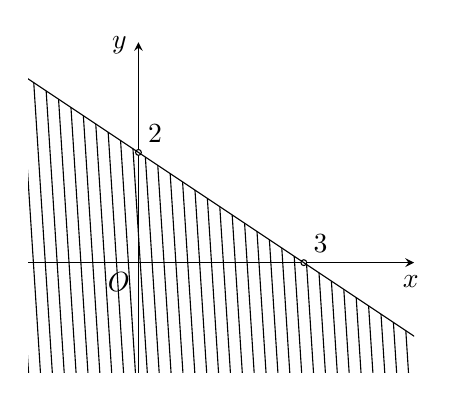
\begin{tikzpicture}[>=stealth,smooth,samples=100,scale=.7]
				\tikzset{declare function={xmin=-2;xmax=5;ymin=-2;ymax=4;},
					smooth,samples=450
				}
				\draw[->] (xmin,0)--(xmax,0) node[shift={(-100:7pt)},font=\normalsize]{$ x $};
				\draw[->] (0,ymin)--(0,ymax) node[shift={(190:7pt)},font=\normalsize]{$ y $};
				\fill (0,0) node[shift={(-135:10pt)},font=\normalsize]{$ O $};
				\draw[fill=white] (3,0)node[above right]{$3$} circle (1.5pt) 
				(0,2) node[above right]{$2$}circle (1.5pt);
				\begin{scope}
				\clip (xmin,ymin) rectangle (xmax,ymax);
				\pgfmathsetmacro{\goc}{abs(atan(0.666))-120}
				\foreach \i in {-10,-9.775,...,10}{
					\draw[black,thin]({\i},{(-2*\i+6)/3})--+(\goc:15);}
				\draw plot[domain=-10:10]({\x},{(-2*\x+6)/3});
				\end{scope}
				\end{tikzpicture}
			\end{center}
		\end{enumerate}	
	}
\end{ex}
\begin{ex}%[0D2V1-3]
	Nhân ngày Quốc tế Thiếu Nhi 1-6, một rạp chiếu phim phục vụ các khán giả một bộ phim hoạt hình. Vé được bán ra có hai loại:
	\begin{itemize}
		\item Loại 1 (dành cho trẻ từ 6-13 tuổi): 50 000 đồng/vé.
		\item  Loại 2 (dành cho người trên 13 tuổi): 100 000 đồng/vé.
	\end{itemize}
	Người ta tính toán rằng, để không phải bù lỗ thì số tiền vé thu được ở rạp chiếu phim này phải đạt tối thiểu 20 triệu đồng. Hỏi số lượng vé bán được trong những trường hợp nào thì rạp chiếu phim phải bù lỗ?
	\loigiai{
		\immini{Gọi $x$ là số lượng vé loại 1 bán được, $y$ là số lượng vé loại 2 bán được $(x,y \in \mathbb{N})$.
			\begin{itemize}
				\item  Số tiền bán vé thu được là $50x+100y$ (nghìn đồng).
				\item  Người ta sẽ phải bù lỗ trong trường hợp $50x+100y<20 000$ hay $x+2y<400 \quad (1)$.
			\end{itemize}
			Miền nghiệm của (1) là những điểm có tọa độ nguyên nằm trong tam giác $OAB$. Vậy, nếu bán được $x$ vé loại 1 và $y$ vé loại 2 mà điểm $(x;y)$ nằm trong tam giác $OAB$ thì rạp phim phải bù lỗ.}{
			\begin{tikzpicture}[line join=round, line cap=round, >=stealth,font=\footnotesize, scale=0.5]
			\draw [pattern=dots,pattern color=myblue] (-3,3.5)--(5,3.5)-- (5,-0.5)--cycle;
			\draw[samples=100,smooth,domain=5:-3,red] plot(\x,{-0.5*(\x)+2})node[above] {$d$};
			\draw [color=white] (-3,3.5)--(5,3.5)-- (5,-0.5);
			\draw[->](-3,0)--(5.2,0) node[right] {$x$};
			\draw[->](0,-1)--(0,3.7) node[right] {$y$};
			\node (0,0) [below left]{$ O $};
			\foreach \x in {-2,...,3}
			\draw[shift={(\x,0)},color=black] (0pt,2pt) -- (0pt,-2pt);
			\foreach \y in {1,...,2}
			\draw[shift={(0,\y)},color=black] (2pt,0pt) -- (-2pt,0pt);
			\node[left] at (0,1.8) {$200$};
			\node[below] at (3.8,0) {$400$};
			\node[right] at (0,2.2) {$A$};
			\node[above] at (4.1,0) {$B$};
			\end{tikzpicture}
		}	
	}
\end{ex}

\begin{ex}%[0D2V1-3]%
	[SGK Toán 10 - Kết nối tri thức]
	Một rạp chiếu phim $2$D phục vụ khán giả một bộ phim mới với $2$ loại vé khác nhau. Vé loại $1$ (từ thứ $2$ đến thứ $5$) giá $80\,000$ đồng/vé, vé loại $2$ (từ thứ $6$ đến chủ nhật và ngày lễ) giá $100\,000$ đồng/vé. Để không phải bù lỗ thì số tiền vé thu được ở rạp chiếu phim này phải đạt tối thiểu $150$ triệu đồng. Hỏi số lượng vé bán được trong những trường hợp nào thì rạp chiếu phim phải bù lỗ?
	\loigiai{
		Gọi $x$, $y$ lần lượt là số vé loại $1$, loại $2$ bán được ($x, y\in\mathbb{N}$).\\
		Tổng số tiền bán vé là $80x+100y$ nghìn đồng.\\
		Rạp chiếu phim phải bù lỗ trong trường hợp số tiền bán vé nhỏ hơn $150$ triệu đồng, tức là 
		\[80x+100y<150\,000\Leftrightarrow 4x+5y<7500.\quad\quad (1)\]
		\immini{
			Miền nghiệm của bất phương trình (1) được xác định như sau
			\begin{itemize}
				\item 	Vẽ đường thẳng $d\colon 4x+5y=7500$.
				\item Chọn gốc tọa độ $O(0;0)$ và tính $4\cdot0+5\cdot0<7500$.\\
			\end{itemize}
			Do đó miền nghiệm của bất phương trình (1) là nửa mặt phẳng bờ $d$, chứa gốc tọa độ $O$, không kể đường thẳng $d$.\\
			Gọi $A$, $B$ lần lượt là giao điểm của $d$ và $Ox$, $Oy$. Khi đó, nếu bán được $x$ vé loại $1$ và $y$ vé loại $2$ mà điểm $(x;y)$ nằm trong miền tam giác $OAB$ không kể cạnh $AB$ thì rạp chiếu phim sẽ phải bù lỗ.
		}
		{
			\begin{tikzpicture}[scale=.7,>=stealth]
			\draw[->] (0,0) -- (5.3,0)node[below]{$x$};
			\draw[->,color=black] (0,0) -- (0,5.3)node[left]{$y$};
			\node[below left] at (0,0){$O$};
			\node[left] at (0,3){$1500$};
			\node[above right] at (0,3){B};
			\node[below] at (4,0){$1875$};
			\node[above] at (4,0){A};
			\clip(0,0) rectangle (5.3,5.3);
			\fill[pattern=north east lines](4,0)-- (5.3,0) -- (5.3,5.3) -- (0,5.3)--(0,3)-- cycle;
			\draw[line width=1.2pt,smooth,samples=100,domain=0:4] plot(\x,{-0.75 *(\x) +3});
			\end{tikzpicture}
		}	
	}
\end{ex}
\begin{ex}%[0D2H1-2]
	Gọi $S$ là tập hợp các giá trị nguyên của tham số $m$ trong đoạn $[-10;10]$ sao cho $(x;y)=(1;-1)$ là nghiệm của bất phương trình $\dfrac{m}{2}x-(m+1)y+2\geq 0$. Tính tổng các phần tử của $S$.
	\loigiai{
		Ta có $(x;y)=(1;-1)$ là nghiệm của bất phương trình $\dfrac{m}{2}x-(m+1)y+2\geq 0$ khi và chỉ khi
		\[\dfrac{m}{2}-(m+1)(-1)+2\geq 0\Leftrightarrow \dfrac{3}{2}m+3\geq 0\Leftrightarrow m\geq -2.\]
		Mà $m\in [-10;10]$ và $m$ nguyên nên $m\in \{-2;-1;\ldots;10\}$.\\
		Do đó tổng các phần tử của $S$ là $(-2)+(-1)+\ldots +10=52$.
	}
\end{ex}
\begin{ex}%[0D2H1-3]%
	[SGK Toán 10 - Kết nối tri thức]
	Ông An muốn thuê một chiếc ô tô (có lái xe) trong một tuần. Giá thuê xe(ngìn đồng/ngày) được cho như bảng sau:
	\begin{center}
		\begin{tabular}{|c|c|c|}
			\hline
			& Phí cố định& Phí tính theo quãng đường di chuyển\\
			\hline
			Từ thứ Hai đến thứ Sáu	& $900$  & $8$ \\
			\hline
			Thứ Bảy và Chủ nhật	& $1\,500$  & $10$  \\
			\hline
		\end{tabular}
	\end{center}
	\begin{enumerate}
		\item Gọi $x$ và $y$ lần lượt là số kilômét ông An đi trong các ngày từ thứ Hai đến thứ Sau và tỏng hai ngày cuối tuần. Viết bất phương trình biểu diễn mỗi liên hệ giữa $x$ và $y$ sao cho tổng số tiền ông An phải trả không vượt quá $14$ triệu đồng.
		\item Biểu diễn miền nghiệm của bất phương trình trên mặt phẳng toạ độ.
	\end{enumerate}
	\loigiai{
		\begin{enumerate}
			\item Ta có $14$ triệu $=14\, 000$ (nghìn đồng).\\
			Số tiền ông An đi $x$ km trong các ngày từ thứ Hai đến thứ Sáu là $900\cdot 5+8x$ (nghìn đồng).\\
			Số tiền ông An đi $y$ km trong hai ngày cuối tuần là $1\,500\cdot 2+10y$ (nghìn đồng).\\
			Số tiền ông An đi trong một tuần là $7\,500+8x+10y$ (nghìn đồng).\\
			Vì số tiền không quá $14$ triệu đồng nên ta có 
			\[7\,500+8x+10y\leq 14\,000\Leftrightarrow 4x+5y\leq 3250.\]
			Vậy bất phương trình cần tìm là $4x+5y\leq 3250$.
			\item Biểu diễn miền nghiệm là 
			\begin{center}
				\begin{tikzpicture}[line join=round, line cap=round, >=stealth,font=\footnotesize, scale=0.5]
				\draw [pattern=dots,pattern color=myblue] (-3,3.5)--(5,3.5)-- (5,-0.5)--cycle;
				\draw[samples=100,smooth,domain=5:-3,red] plot(\x,{-0.5*(\x)+2})node[above] {$d$};
				\draw [color=white] (-3,3.5)--(5,3.5)-- (5,-0.5);
				\draw[->](-3,0)--(5.2,0) node[right] {$x$};
				\draw[->](0,-1)--(0,3.7) node[right] {$y$};
				\node (0,0) [below left]{$ O $};
				\node[left] at (0,1.8) {$650$};
				\node[below] at (3.8,0) {$812{,}5$};
				\node[right] at (0,2.2) {$A$};
				\node[above] at (4.1,0) {$B$};
				\end{tikzpicture}
			\end{center}
			Bước 1: Vẽ đường thẳng $4x+5y=3250$ (nét liền).\\
			Bước 2: Thay toạ độ điểm $O(0;0)$ vào biểu thức $4x+5y$ ta được $4\cdot 0+5\cdot 0=0<3250$. Điểm $O$ thuộc miền nghiệm.\\
			Vậy miền nghiệm là nửa mặt phẳng bờ là đường thẳng $4x+5y=3250$ và chứa gốc toạ độ và $(x;y)$ nằm trong miền tam giác $OAB$ kể cả đoạn $AB$.
		\end{enumerate}
	}
\end{ex}
\begin{ex}%[0D2H1-3]%
	[THPT Nguyễn Công Trứ - Tp. HCM - GHKI-NH23-24]
	Bạn An cần làm hai loại mô hình bằng giấy bìa cứng. Để làm một mô hình loại $\mathrm{I}$ cần dùng $5$ tấm bìa cứng; để làm một mô hình loại $\mathrm{II}$ chỉ cần dùng $2$ tấm bìa cứng. Gọi $x$ và $y$ lần lượt là số mô hình loại $\mathrm{I}$ và $\mathrm{II}$ mà bạn An có thể làm được. Biết rằng hiện bạn An chỉ còn $10$ tấm bìa cứng. Hãy lập các bất phương trình mô tả số mô hình loại $\mathrm{I}$ và $\mathrm{II}$ mà bạn An có thể làm được. Biểu diễn miền nghiệm của các bất phương trình đó trên cùng một mặt phẳng toạ độ $Oxy$.
	\loigiai{
		\immini{
			Gọi $x$ và $y$ lần lượt là số mô hình loại $\mathrm{I}$ và $\mathrm{II}$ mà bạn An có thể làm được.\\
			Theo giả thiết bài toán, các bất phương trình mô tả số mô hình loại $\mathrm{I}$ và $\mathrm{II}$ mà bạn An có thể làm được thỏa hệ sau $$\heva{&x\ge0\\&y\ge0\\&5x+2y\le 10}$$
			Gọi đường thẳng $(d):5x+2y=10$.\\
			Miền nghiệm của các bất phương trình trên là miền tam giác không bị gạch, kể cả các cạnh.
		}{
			\begin{tikzpicture}[scale=0.5,>=stealth, font=\footnotesize, line join=round, line cap=round]
			\draw[->](-1,0)--(4,0) node[below] {$x$};
			\draw[->](0,-1)--(0,8) node[left] {$y$};
			\node (0,0) [below left]{$ O $};
			\foreach \x in {-1,...,2}
			\draw[shift={(\x,0)},color=black] (0pt,2pt) -- (0pt,-2pt);
			\foreach \y in {1,...,5}
			\draw[shift={(0,\y)},color=black] (2pt,0pt) -- (-2pt,0pt);
			\draw[samples=100,smooth,red,domain=-1:2.4] plot(\x,{5-2.5*(\x)});
			\fill[pattern=north west lines,pattern color=blue] (-1,7.5)--(3.5,7.5)--(3.5,-1)--(2.4,-1)--cycle;
			\fill[pattern=north east lines,pattern color=yellow] (-1,-1)--(-1,7.5)--(0,7.5)--(0,-1)--cycle;
			\fill[pattern=north east lines,pattern color=brown] (-1,0)--(3.5,0)--(3.5,-1)--(-1,-1)--cycle;
			\foreach \i in {2}{\draw[fill=black] (\i,0) circle(1pt) node[below]{$\i$};}
			\foreach \i in {5}{\draw[fill=black] (0,\i) circle(1pt) node[left]{$\i$};}
			
			\end{tikzpicture}}
	}
\end{ex}
\begin{ex}%[0D2V1-2]
	Cho tam giác $ABC$ có $A(0;3)$, $B(-1;2)$, $C(2;1)$. Tìm điều kiện của tham số $m$ để điểm $M\left(m;\dfrac{2m-1}{2}\right)$ nằm trong tam giác $ABC$?	
	\loigiai{
		Đường thẳng $AB\colon \dfrac{x-0}{-1-0}=\dfrac{y-3}{2-3}\Leftrightarrow x-y+3=0$.\\
		Đường thẳng $AC\colon \dfrac{x-0}{2-0}=\dfrac{y-3}{1-3}\Leftrightarrow x+y-3=0$.\\
		Đường thẳng $BC\colon \dfrac{x-2}{2-(-1)}=\dfrac{y-1}{1-2}\Leftrightarrow x+3y-5=0$.\\
		Điều kiện cần và đủ để điểm $M$ nằm bên trong tam giác $ABC$ là điểm $M$ cùng với  mỗi đỉnh $A$, $B$, $C$ lần lượt cùng phía với nhau đối với cạnh $AB$, $AC$, $BC$ tức là
		\[\heva{& (1\cdot0+3\cdot 3-5)\left(1\cdot m+3\cdot \dfrac{2m-1}{2}-5\right)>0\\& (1\cdot (-1)+1\cdot 2-3)\left(1\cdot m+1\cdot \dfrac{2m-1}{2}-3\right)>0\\& (1\cdot 2-1\cdot 1+3)\left(1\cdot m-1\cdot \dfrac{2m-1}{2}+3\right)>0}\Leftrightarrow \heva{& m>\dfrac{13}{8}\\& m<\dfrac{7}{4}\\& 14>0}\Leftrightarrow \dfrac{13}{8}<m<\dfrac{7}{4}.\]	
		Vậy với $\dfrac{13}{8}<m<\dfrac{7}{4}$ sẽ thoả mãn yêu cầu bài toán.
	}
\end{ex}
\begin{ex}%[0D2H1-3]%
	[SGK Toán 10 - Cánh Diều]
	Trong $1$ lạng ($100$ gram) thịt bò chứa khoảng $26$ gram protein, $1$ lạng cá rô phi chứa khoảng $20$ gram protein. Trung bình trong một ngày, một người phụ nữ cần tối thiểu $46$ gram protein. Gọi $x$, $y$ lần lượt là số lạng thịt bò và số lạng cá rô phi mà một người phụ nữ nên ăn trong một ngày. Bất phương trình bậc nhất hai ẩn $x$, $y$ để biểu diễn lượng protein cần thiết cho một người phụ nữ trong một ngày có dạng $ax+by\geq 23$ với $a$, $b$ là các số dương. Tính $T=\dfrac{2016}{13}a+b$. 
	\loigiai{
		\begin{itemize}
			\item Lượng protein có trong $x$ lạng thịt bò và $y$ lạng cá rô phi là $26x+20y$ (gram).
			\item Vì lượng protein tối thiểu là $46$ gram nên ta có $26x+20y\geq 46\Leftrightarrow 13x+10y\geq 23$.
		\end{itemize}
		Từ đó suy ra $a=13$, $b=10$ vậy $T=2026$.
	}
\end{ex}
\begin{ex}%[0D2V1-3]%
	[SBT Toán 10 - Kết nối tri thức]
	Một cửa hàng bán lẻ bán hai loại hạt cà phê. Loại thứ nhất giá $140$ nghìn đồng/kg và loại thứ hai giá $180$ nghìn đồng/kg. Cửa hàng trộn $x$ kg loại thứ nhất và	$y$	kg loại thứ hai sao cho hạt cà phê đã trộn có giá không quá $170$ nghìn đồng/kg.
	\begin{enumerate}
		\item Viết bất phương trình bậc nhất hai ẩn $x$, $y$ thoả mãn điều kiện đề bài.
		\item Biểu diễn miền nghiệm của bất phương trình tìm được ở câu a trên mặt phẳng toạ độ.
	\end{enumerate}
	\loigiai{
		\begin{enumerate}
			\item Theo đề bài ta có $140x+180y\leq 170(x+y)\Leftrightarrow 3x-y\geq 0$.
			\item Biểu diễn miền nghiệm của bất phương trình $3x-y\geq 0$.
			\begin{center}
				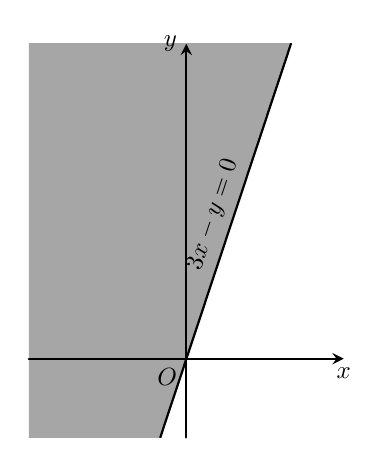
\begin{tikzpicture}[line join=round, line cap=round,>=stealth,thick]
				\tikzset{every node/.style={scale=0.9}}
				\begin{scope}
				\clip (-2,-1) rectangle (2,4);
				\fill[black!35] (-3,-9)--(-3,9)--(3,9)--cycle;
				\draw (1.33,4)--(-0.33,-1) node [pos=0.45, above, sloped] {$3x-y=0$};
				\end{scope}
				\draw[->] (-2,0)--(2,0) node[below]{$x$};
				\draw[->] (0,-1)--(0,4) node[left]{$y$};
				\draw (0,0) node[below left]{$O$};
				\end{tikzpicture}
			\end{center}
			\begin{itemize}
				\item Vẽ đường thẳng $d\colon 3x-y=0$ trên mặt phẳng toạ độ.
				\item Lấy điểm $M(1;0)$ không thuộc $d$ và điểm $M$ thoả mãn $3\cdot 1-0=3>0$. Do đó, miền nghiệm của bất phương trình là nửa mặt phẳng bờ $d$ chứa điểm $M(1;0)$.
			\end{itemize}
		\end{enumerate}
	}
\end{ex}
\begin{ex}%[0D2V1-2]
	Cho bất phương trình $2x+3y-10\leq 0$. Hỏi có bao nhiêu cặp số nguyên $(m_0;n_0)$ thoả mãn $(m_0^2;n_0^2)$ là nghiệm của bất phương trình đã cho?
	\loigiai{
		Vì $(m_0^2;n_0^2)$ là nghiệm của bất phương trình $2x+3y-10\leq 0$ nên ta có 
		\[2m_0^2+3n_0^2\leq 10\Rightarrow \heva{& m_0^2\leq 5\\& n_0^2\leq \dfrac{10}{3}}\Leftrightarrow \heva{& -\sqrt{5}\leq m_0\leq \sqrt{5}\\& -\sqrt{\dfrac{10}{3}}\leq n_0\leq \sqrt{\dfrac{10}{3}}}.\]
		Do $m_0$, $n_0$ là số nguyên nên $\heva{& m_0\in \{-2;-1;0;1;2\}\\& n_0\in \{-1;0;1\}}$. Suy ra có $15$ cặp số thỏa mãn.\\
		Thử lại ta loại các bộ $(2;-1)$, $(2;1)$; $(-2;1)$, $(-2;-1)$.\\
		Vậy có $11$ cặp số $(m_0;n_0)$ sao cho $(m_0^2;n_0^2)$ là nghiệm của bất phương trình đã cho.
	}	
\end{ex}
\begin{ex}%[0D2V1-3]
	Một cửa hàng chuẩn bị tổ chức chương trình khuyến mãi dịp hè. Họ có kế hoạch chi không quá $10$ triệu đồng để in tờ rơi quảng cáo và áp phích treo tường.
	\begin{itemize}
		\item Chi phí in $1$ tờ rơi là $2\,000$ đồng.
		\item Chi phí in $1$ áp phích là $20\,000$ đồng.
	\end{itemize}
	Gọi $x$, $y$ lần lượt là số từ rơi, số tờ áp phích được in. Với $x=3\,000$ hãy tính giá trị lớn nhất có thể in áp phích để điều kiện chi phí thoả mãn.
	\loigiai{
		Chi phí in $x$ tờ rơi quảng cáo là $2x$ (nghìn đồng).\\
		Chi phí in $y$ tờ áp phích là $20y$ (nghìn đồng).\\
		Tổng chi phí in là $2x+20y$ (nghìn đồng). Theo gải thiết thì chi phí in không quá $10$ triệu đồng nên ta có
		\[2x+20y\leq 10\,000\Leftrightarrow x+10y\leq 5\,000.\]
		Thay $x=3\,000$ vào bất phương trình
		\[3\,000+10y\leq 5\,000\Rightarrow 10y\leq 2\,000\Rightarrow y\leq 200.\]
		Vậy giá trị lớn nhất có thể in áp phích là $y=200$.
	}
\end{ex}
\begin{ex}%[0D2V1-2]%
	[Tài liệu Thầy Đạng Mạnh Hùng - Bắc Ninh-NH24-25]
	Trong hệ trục toạ độ $Oxy$, cho bất phương trình $2x+y\geq 2$ có miền nghiệm $D$. Dựng hình vuông $ABCO$ có cạnh $a$ nằm trong góc phần tư thứ nhất, với $O(0;0)$ là gốc toạ độ. Biết rằng diện tích phần chung giữa miền nghiệm $D$ và hình vuông $ABCO$ bằng $2025$. Tìm $a$.
	\loigiai{
		\immini{Vẽ đường thẳng $d\colon 2x+y=2$.\\
			Thay điểm $O(0;0)$ vào bất phương trình $2x+y\geq 2$ ta được $0\geq 2$ (vô lí) nên điểm $O(0;0)$ không thuộc miền nghiệm $D$ của bất phương trình $2x+y\geq 2$.\\
			Khi đó miền nghiệm $D$ của bất phương trình $2x+y\geq 2$ là miền không chứa điểm $O(0;0)$ có bờ $d$, kể cả đường thẳng $d$ (miền không gạch như hình vẽ).\\
			Vẽ hình vuông $ABCO$ bằng cạnh $a$ nằm trong góc phần tư thứ nhất trên cùng hệ trục toạ độ với miền nghiệm $D$.\\
			Dựa vào hình vẽ ta thấy diện tích phần chung giữa miền nghiệm $D$ và hình vuông (phần tô màu) là
			\begin{eqnarray*}
				S&=&S_{ABCO}-S_{OEF}=OA^2-\dfrac{1}{2}\cdot OE\cdot OF\\
				&=&a^2-\dfrac{1}{2}\cdot 2\cdot 1\\
				&=& a^2-1.
			\end{eqnarray*}
			Mà $S=2025$ nên $a^2-1=2025\Leftrightarrow a^2=2026\Leftrightarrow a=\sqrt{2026}$.\\
			Vậy $a=\sqrt{2026}$.
		}{
			\begin{tikzpicture}[scale=.7, font=\footnotesize, line join=round, line cap=round, >=stealth]
			
			\begin{scope}
			\clip (-2,-2) rectangle (5,5);
			\fill[black!35] (-3,8)--(-3,-10)--(6,-10)--cycle;
			\draw (-1.5,5)--(2,-2) node [pos=0.2, above, sloped] {$2x+y-2=0$};
			\end{scope}
			\draw[->] (-2,0)--(5,0) node[below]{$x$};
			\draw[->] (0,-2)--(0,5) node[left]{$y$};
			\draw (0,0) node[below left]{$O$};
			\path 
			(0,0) coordinate (O)
			(4,0) coordinate (A)
			(4,4) coordinate (B)
			($(O)+(B)-(A)$) coordinate (C)
			(0,2) coordinate (E)
			(1,0) coordinate (F)
			;
			\foreach \x in {1}
			\draw[thin] (\x,1pt)--(\x,-1pt) node [below] {$\x$};
			\foreach \y in {2}
			\draw[thin] (1pt,\y)--(-1pt,\y) node [left] {$\y$};
			\draw (A)--(B)--(C);
			\fill[blue, opacity=0.5] (A)--(B)--(C)--(E)--(F)--cycle;
			\foreach \x/\g in {A/-90,B/0,C/180,E/20,F/70}\fill[black] (\x) circle (1pt)+(\g:.3)node{$\x$};
			\end{tikzpicture}
		}
	}
\end{ex}